\subsection{Overview}

This section describes the functionality and construction of the MAP Electronics Control Unit (ECU) which is generally responsible for motion control, data acquisition, and communication with peripheral systems as well as the host computer. The following chapter treats the hardware and microcontroller firmware components as two distinct but interrelated subsystems.

%---------------------------------------------------------


\subsection{Hardware}

\subsubsection{Suggested Reading}

\paragraph{Microcontroller}

\begin{itemize}

    \item \href{https://www.st.com/resource/en/user_manual/dm00499171-stm32h7-nucleo144-boards-mb1363-stmicroelectronics.pdf}{STM32H7 Nucleo-144 boards (MB1363) - User manual}
    
    \item \href{https://www.st.com/resource/en/datasheet/stm32h7a3ai.pdf}{Datasheet - STM32H7A3xI/G - 32-bit Arm Cortex}

\end{itemize} 

\paragraph{Motor Drivers}

\begin{itemize}
    
    \item \href{https://www.trinamic.com/fileadmin/assets/Products/ICs_Documents/TMC2130_datasheet.pdf}{TMC2130 Datasheet}
    
    \item \href{https://en.wikipedia.org/wiki/Serial_Peripheral_Interface}{Serial Peripheral Interface - Wikipedia}
    
\end{itemize}



\subsubsection{Introduction}

The following section describes the structure, connections, and roles of the different electrical components which together constitute hardware aspect of the Primary ECU. A schematic of the system can be seen in figure \ref{fig:ECU} below. 

\begin{figure}
\centering
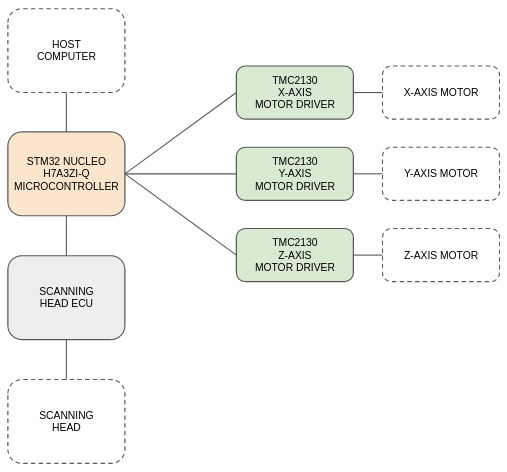
\includegraphics[width=0.8\textwidth]{Primary-ECU/figs/ECU-overview.png}
\caption{\label{fig:ECU}The structure of the Primary ECU.}
\end{figure}

Broadly speaking, the system consists of motor drivers, a high-performance STM32 NUCLEO-H7A3ZI-Q microcontroller development board for the control firmware, and the interchangeable Scanning Head ECU’s specific to a given acquisition technique. By way of example, the XRF Electronics Control Unit additionally contains a constant current source for the helium flow solenoid valve, a driver circuit for the ultrasonic distance sensor, and an Artix-7 FPGA onto which the digital pulse processing (DPP) firmware is implemented. The structures and functions of each individual Scanning Head ECU are all detailed in the dedicated chapters.

\subsubsection{Microcontroller}

The central microcontroller (MCU) within the ECU performs four primary functions: to receive and act upon high-level commands issued by the host computer, to receive and parse data from the acquisition hardware, to send this data to the host computer, and finally to interface with the motion control platform. These functions are each implemented as “tasks” or threads operating concurrently on the MCU. The details of this can be found in the “Firmware” section of this chapter.

The MCU employed in the system is a single-core STM32H7A3ZI M7 ARM processor installed on a NUCLEO-H7A3ZI-Q development board. This processor features a maximum clock speed of 280 MHz, 2 MB of flash memory, and 1376 KB of SRAM. Ideally, a higher specification dual-core MCU such as that employed on the NUCLEO-H743ZI2 would be used instead, however owing to the global chip shortage these were not available.

Interfacing between the MCU and the various components occurs via the IO pins in the case of the Scanning Head ECU’s and motor drivers, and the on-board USB connection in the case of the host computer. The exact connections with the IO pins are laid out in the “Motor Drivers” section below as well as in the Scanning Head ECUs chapter.


\subsubsection{Scanning Head Electronic Control Units}

The Scanning Head ECUs (SHECUs) are swappable modules which contain the electronics necessary to interface between the central MCU and a given scanning head. The purpose of which is ultimately to facilitate the control of the components present on the scanning head as well as to receive, process, and transmit data to the central MCU.

By way of example, the XRF Electronics Control Unit contains a driver circuit for the helium flow solenoid valve, a driver circuit for the ultrasonic distance sensor, and an FPGA onto which the digital pulse processing firmware is implemented.

To the greatest extent possible, connections on the MCU have been shared across as many SHECUs as possible within the constraints imposed by the task-specific mapping of pins within the firmware - such as those coupled to hardware timers, for instance. The goal of which is to minimise the number of conductors necessary to interface the MCU with the SHECUs and to simplify the wiring.
As mentioned previously, the specifics of each SHECU are covered in their respective chapters.


\subsubsection{Motor Drivers}

The ECU features three TMC2130 bi-polar stepper motor drivers which are each responsible for driving a single axis/motor. They receive instructions from the microcontroller via the common step-direction protocol. Essentially, the voltage on the DIR pin determines the direction of rotation (clockwise or anti-clockwise) and a rising edge on the STEP pin instructs the driver to take a single step in the chosen direction.

Upon startup, the motor drivers receive commands through SPI from the MCU so as to configure the various functionalities of the driver circuit such as the microstepping, the current limits, the shape of the incident pulses, etc. After this initial configuration, the SPI interface can be used to receive performance information and failure warnings from the drivers. The details of all this can be found in the relevant datasheet listed in the “Suggested Reading” section above.

The wiring of the motor drivers to the MCU, the power supplies, and the motors can be seen in figure \ref{fig:motor-MCU} below.

\begin{figure}
\centering
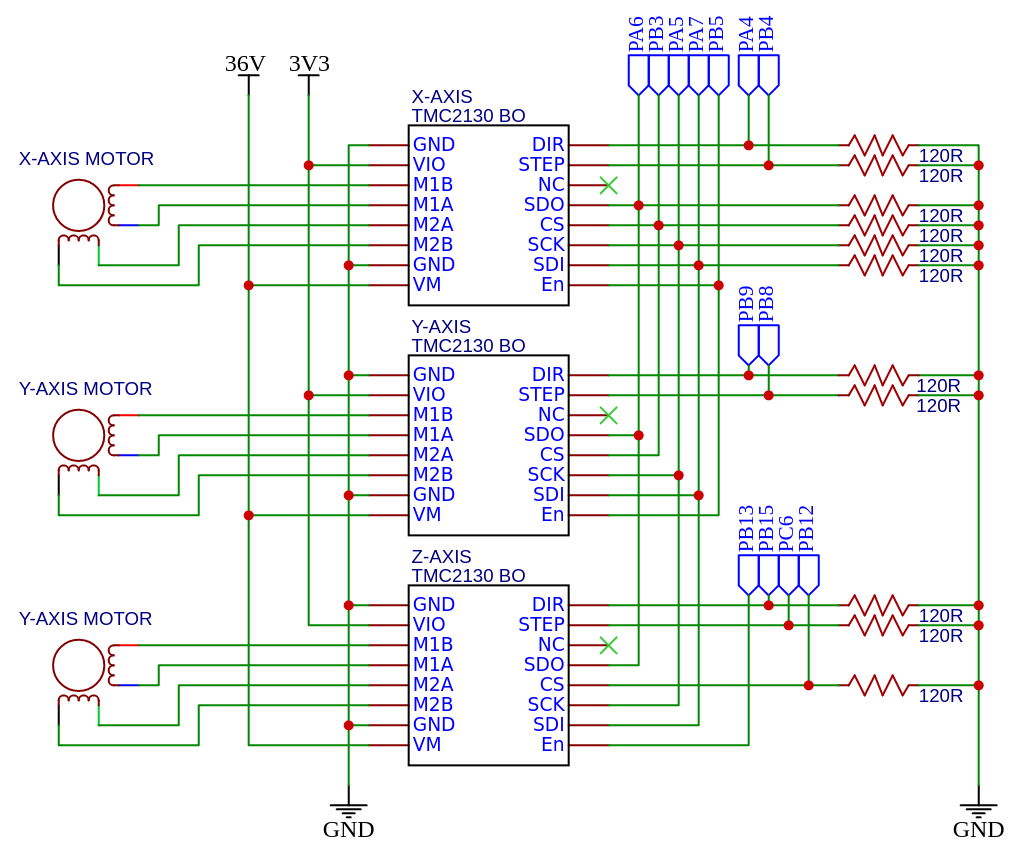
\includegraphics[width=0.8\textwidth]{Primary-ECU/figs/motor-MCU.png}
\caption{\label{fig:motor-MCU}The Connections between the MCU, motor drivers, and motors.}
\end{figure}

Notice that the chip select (CS) and enable (EN) pins for X and Y axis are shorted whereas those on the Z stage are kept separate. This is because the Z stage is responsible for the autofocus and this decoupling allows for its independent configuration should the designer wish to do so.





%---------------------------------------------------------


\subsection{Control Firmware}

\subsubsection{Suggested Reading}

\paragraph{STM32 General}

\begin{itemize}
    

    \item \href{https://www.digikey.com/en/maker/projects/getting-started-with-stm32-introduction-to-stm32cubeide/6a6c60a670c447abb90fd0fd78008697}{Getting Started with STM32 - Introduction to STM32CubeIDE}
    
    \item \href{https://www.digikey.com/en/maker/projects/getting-started-with-stm32-timers-and-timer-interrupts/d08e6493cefa486fb1e79c43c0b08cc6}{Getting Started with STM32 - Timers and Timer Interrupts}
    
    \item \href{https://www.digikey.com/en/maker/projects/getting-started-with-stm32-working-with-adc-and-dma/f5009db3a3ed4370acaf545a3370c30c}{Getting Started with STM32 - Working with ADC and DMA}
    
    \item \href{https://deepbluembedded.com/stm32-adc-read-example-dma-interrupt-polling/}{STM32 ADC Read Example – DMA / Interrupt / Polling}
    
    \item \href{https://deepbluembedded.com/how-to-receive-spi-with-stm32-dma-interrupt/}{How To Receive SPI Data With STM32 DMA / Interrupt / Polling Modes}
    
    \item \href{https://deepbluembedded.com/how-to-receive-uart-serial-data-with-stm32-dma-interrupt-polling/}{How To Receive UART Serial Data With STM32 - DMA / Interrupt / Polling}
    
    \item \href{https://deepbluembedded.com/stm32-timers-tutorial-hardware-timers-explained/}{STM32 Timers Explained Tutorial - Timer Modes Examples, Interrupts, and PWM}
    
    \item \href{https://www.st.com/resource/en/application_note/dm00236305-generalpurpose-timer-cookbook-for-stm32-microcontrollers-stmicroelectronics.pdf}{STM32 General Purpose Timer Cookbook}

\end{itemize}

\paragraph{FreeRTOS, Queues, Semaphores, etc.}

\begin{itemize}
    
    \item \href{https://en.wikipedia.org/wiki/Real-time_operating_system}{Real-time operating system - Wikipedia}
    
    \item \href{https://www.freertos.org/features.html}{Official FreeRTOS Documentation}
    
    \item \href{https://www.codeinsideout.com/blog/stm32/free-rtos/interrupt/}{Interrupt - STM32 - FreeRTOS - Code Inside Out}

\end{itemize}



\paragraph{STM32 Nucleo H7A3ZI-Q Board and MCU}

\begin{itemize}


    \item \href{https://www.st.com/resource/en/user_manual/dm00499171-stm32h7-nucleo144-boards-mb1363-stmicroelectronics.pdf}{STM32H7 Nucleo-144 boards (MB1363) - User manual}
    
    \item \href{https://www.st.com/resource/en/datasheet/stm32h7a3ai.pdf}{Datasheet - STM32H7A3xI/G - 32-bit Arm Cortex}
    
\end{itemize}


\paragraph{Motor Drivers}

\begin{itemize}

    \item \href{https://en.wikipedia.org/wiki/Serial_Peripheral_Interface}{Serial Peripheral Interface - Wikipedia}

    \item \href{https://www.trinamic.com/fileadmin/assets/Products/ICs_Documents/TMC2130_datasheet.pdf}{TMC2130 Datasheet}

\end{itemize} 



\subsubsection{Introduction}

This section describes the construction and function of the main control firmware implemented on the STM32H7A3ZI MCU. As mentioned previously, this firmware was designed to operate on a single chip and in doing so, to handle all of the computational tasks required by the system. This approach of having multiple tasks all running simultaneously on the same MCU (as opposed to multiple MCU’s running dedicated tasks) has the advantage of greatly reducing the complexity of the system from both a hardware and firmware standpoint, facilitates the ready diagnosis and repair of bugs, and promotes modularity. The disadvantage is that the chosen MCU has to be exceptionally powerful in order to reliably perform these tasks and additional care must be paid to the design of the firmware so as to not overload the processor.

The STM32CubeIDE development environment was used both to configure the STM32 microcontroller unit (MCU) along with its peripherals (the ADC, SPI, UART, etc.), as well as to write the actual firmware, which was done in C.

In order to handle the array of tasks that must all run concurrently, a Real Time Operating System (RTOS) was used. Broadly speaking, an RTOS is a piece of software which directs resources to permit effective simultaneity in the operation of tasks or threads (these are analogous terms). A single core on any processor is only capable of running one task at a time and as such the appearance of simultaneity is accomplished by rapidly switching between these tasks. Additionally, the MCU is configured in such a way as to minimise the reliance on the CPU using interrupts, Direct Memory Access (DMA), and through the use of modules present on the chip but separate to the CPU such as timers.

Broadly speaking the MAP Control firmware consists of a series of variable and structure declarations, function initialisations, configuration functions, task functions, and Interrupt Service Routines (ISR). The roles of which will be discussed in subsequent sections.



\subsubsection{High Level Commands}

The high level commands used to operate the CHMAP are summarised in figure \ref{fig:high-level-commands}. These commands are issued to the MCU within the Primary ECU which then acts to execute the required action by the interfacing with the relevant hardware components.

\begin{figure}
\centering
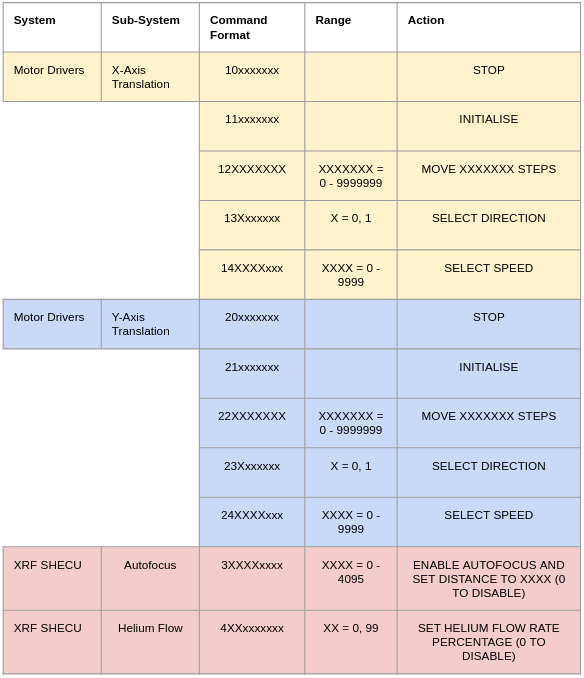
\includegraphics[width=1.0\textwidth]{Primary-ECU/figs/command-table.png}
\caption{\label{fig:high-level-commands}The commands available to the host computer. Note than an upper-case 'X' denotes a meaningful character, whereas a lower-case 'x' can be any UTF-8 character without affecting the issued command.}
\end{figure}

As can be seen, each command consists of 9 characters - the leftmost of which is the most significant and determines the target system; '1' for x-axis motor, '2' for y-axis motor, etc. If a series of different command types exist within a single sub-system, these are addressed with the second most significant digit. In this way, the tree of commands is navigated with increasing specificity by moving from left to right along the 9 digit command structure.

The remaining digits either encode information such as states and variables (represented by an upper-case 'X' in figure \ref{fig:high-level-commands}) or can take any value without affecting the command (denoted by a lower case 'x'). It is important however that the host computer always issued commands \textit{exactly} 9 bytes long or the UART buffer present in the MCU will overflow and unpredictable behaviour will result.

Upon the receipt of a command, the MCU will respond by sending the received command back to the host computer in order to verify that it was successfully received.



\subsubsection{Configuration}

The configuration of the MCU and it's various hardware peripherals (timers, analogue-to-digital converters, communications, etc.) is performed within the STM32CubeIDE as per the material listed in the \textit{Suggested Reading} above. The details of this configuration can be found in table \ref{tab:MCU-config}.

\begin{table}
\centering

\begin{tabular}{|l|l|l|}
\hline
\thead{Function}                                            & \thead{Peripheral}             & \thead{Notes} \\\hline

\small\makecell{UART Communication\\ with Host Computer}    & \small\makecell{USART3}           & \small\makecell{Baud Rate 115200 bits/s} \\\hline

\small\makecell{SPI Communication\\ with Motor Drivers}     & \small\makecell{SPI1}             & \small\makecell{Full-duplex master \\ 8 bit (40 total bits) \\ No interrupt or DMA \\\\ Prescaler 128 \\\\ CPOL High \\ CPHA 2 Edge}  \\\hline

\small\makecell{Autofocus}                                  & \small\makecell{ADC1 \\ TIM3}     & \small\makecell{IN2 Single-Ended \\ 12 bit Resolution \\ Single Acquisition \\ Interrupt on ADC1}  \\\hline

\small\makecell{Motor Pulse Timer}                          & \small\makecell{TIM5}             & \small\makecell{TIM5 Global Interrupt \\ Internal Clock \\\\ PSC 0 \\ ARR 70000-1} \\\hline

\small\makecell{RTOS}                                       & \small\makecell{FREERTOS}         & \small\makecell{CMSIS V1 \\ Everything else default \\ The CMSIS wrapper is NOT used \\\\ Timebase source for HAL \\ changed to TIM6} \\\hline

\small\makecell{SPI Communication\\ with DPP}               & \small\makecell{SPI2}             & \small\makecell{Full-duplex Slave \\ 16 bit \\\\ DMA1 Channel 4, Priority Medium \\ Circular \\ Byte \\\\ CPOL Low \\ CPHA 1 Edge} \\\hline

\small\makecell{Solenoid Timer}                             & \small\makecell{TIM2}             & \small\makecell{TIM2 Global Interrupt \\ Internal Clock \\ PWM Generation \\\\ PSC 0 \\ ARR 280000-1 (1KHz)} \\\hline



\end{tabular}
\caption{\label{tab:MCU-config}The configuration of the STM32 MCU and peripherals.}
\end{table}



\subsubsection{Declarations and Initialisations}

Much of the code present within main.c responsible for the configuration of the MCU is automatically generated by the IDE upon the allocation of pins and the configuration of peripherals. For the sake of brevity, these aspects of the code will not be discussed and therefore any syntax not outlined herein can be treated as beyond the responsibility of the user.

Ordinarily, FreeRTOS is implemented in the STM32 through a wrapper/abstraction layer called CMSIS. Being that our firmware does not use this wrapper, the necessary libraries must be included explicitly within the \verb|/* USER CODE BEGIN Includes */| section as shown in \ref{listing:includes}. This approach was chosen as the documentation and support for CMSIS is a great deal weaker than that available for standard FreeRTOS. A disadvantage of this however is that certain sections of automatically generated code must be deleted every time the configuration is changed. Thankfully, once the \verb|#include "CMSIS_V1"| statement is removed, all unnecessary code will show errors and can therefore be identified and deleted.

\begin{listing}
\begin{minted}{c}
/* USER CODE BEGIN Includes */
#include "FreeRTOS.h"
#include "task.h"
#include "timers.h"
#include "queue.h"
#include "semphr.h"
#include "event_groups.h"

#include <stdio.h>
#include <stdlib.h>
#include <stdbool.h>
#include "string.h"
/* USER CODE END Includes */
\end{minted}
\label{listing:includes}
\end{listing}

Next, buffers for the ADC and Digital Pulse Processor data reception are initialised under \verb|/* USER CODE BEGIN PV */|. These global variables store data shared between tasks and ISRs instead of using more complex shared memory structures such as queues. The nature of this approach will be discussed in greater detail in the Interrupt Service Routines section below. Additionally, a series of constants defining the configuration of the motor driver boards are also declared under \verb|\\Motor control registers|.

Under \verb|/* USER CODE BEGIN 0 */| the handles necessary for the initialisation of tasks, queues, and semaphores are declared as are the entry functions for the tasks which are defined explicitly later in \verb|main.c|. The details are largely unimportant and there is little complexity to be found here; just understand that in order to create new tasks/queues/semaphores, they must first be declared here.

The main function begins by setting the output pins to their default values and the calibration of the ADC with the command:


\begin{listing}
\begin{minted}{c}

while(HAL_ADCEx_Calibration_Start(&hadc1, ADC_CALIB_OFFSET, ADC_SINGLE_ENDED) != HAL_OK);

\end{minted}
\label{listing:ADC-calib}
\end{listing}


What follows is the actual creation of the tasks, semaphores, and queues employed within the program. For details regarding the use and utility of these structures, review the FreeRTOS documentation linked above. The Hardware Abstraction Layer (HAL) is invoked to initialise the peripherals in their respective modes (polling, global interrupts, and DMA). The motor controller boards are also configured here using the previously declared variables to define the state of the driver board’s registers. This is by pulsing the relevant chip select (CS) pins and sending the data over SPI. Finally, the FreeRTOS task scheduler is invoked with the command \verb|vTaskStartScheduler()| and the succeeding while loop is therefore never executed.

What follows is a series of hardware initialisation functions generated automatically by the IDE and they should never be changed directly - only ever through the Device Configuration Tool.

Under \verb|/* USER CODE BEGIN 4 */|, there is the real substance of the firmware. That is, the code which describes the tasks and the non-timer related ISRs.

\subsubsection{Tasks}

\paragraph{UARTcom}\\

The role of the \verb|UARTCom| task is both to transmit data to the host computer and to receive commands from the host computer as per figure \ref{fig:high-level-commands}. These commands are buffered into queues for subsequent execution by the relevant task. Queues are used here in order to ensure firstly that no command is lost if a second command is sent prior to the first being executed, and that a command that is being read by a task is not corrupted by simultaneous reception of another command.

The task begins with the declaration of a number of buffers - the role of which will be explained below. The main \verb|while| loop begins with

% Within the main \verb|while| loop we have sections which deal both with the transmission of data from the tasks to the host computer, and the reception of commands from the host computer and its direction towards the task.

\begin{listing}
\begin{minted}{c}

if (xQueueReceive(UARTtxQueue, &UARTtxBuffer, 100) == pdTRUE){
HAL_UART_Transmit(&huart3, (uint8_t *)UARTtxBuffer, sizeof(UARTtxBuffer), 100);
}

\end{minted}
\label{listing:ADC-calib}
\end{listing}

which checks to see if any task has passed information into the \verb|UARTtxQueue| queue for transmission via UART to the host computer. If if this true, then this information is buffered from the queue into \verb|UARTtxBuffer| and sent.

Next the firmware attempts to receive data from the host computer via an interrupt (so as to minimise loading on the processor) and buffer this information into \verb|UARTtxBuffer|. Once the reception of data is complete, a semaphore is given from the \\\verb|HAL_UART_RxCpltCallback| ISR to signal that it is okay to proceed.

This interrupt/ISR/semaphore structure is used throughout the firmware as it is an effective means to prevent the processor from having to poll a peripheral (in this case, the UART) to check for a change of state. Rather, other tasks can be completed and the processor is only notified once a change of state occurs (again in this case, the reception of a command is complete). Furthermore, a task is unable to access the memory in which a variable is held until the interrupt is triggered, preventing corruption.

If a semaphore was given by the ISR, a \verb|switch| statement is invoked which checks the first character of the received command, buffers the meaningful section of the command into a queue, and/or performs some instructions. Beginning with the case in which the first character is a '0', the \verb|MtrStop| flag is triggered, preventing any further motion in any axis. As for the case in which the first character is a '1', it can be seen from figure \ref{fig:high-level-commands} that this refers to commands directed at the X-axis of the 3-Axis Linear Stage. The executed instructions are as follows:

\begin{listing}
\begin{minted}{c}

memcpy(MtrCtrlXrx_temp, UARTrxBuffer + 1, 8);
xQueueSend(MtrCtrlXrxQueue, &MtrCtrlXrx_temp, 100);
break;

\end{minted}
\label{listing:1}
\end{listing}

First, it is checked if a 'STOP' command is issued by seeing if the second character is a '0', and if this is the case the global \verb|MtrStop| variable is set to true. Next, the 8 bytes following the leading '1' are copied into the \verb|MtrCtrlXrx_temp| buffer and send it to the \verb|MtrCtrlXrxQueue| queue for later reception by the \verb|MotorCtrlX| task. This is effectively the exact same process as for the case where the leading character is a '2', except for the Y-axis of the linear stage.

In the case that the leading digit is a '3' (addressing the auto focus):

\begin{listing}
\begin{minted}{c}

memcpy(AutoFocusrx_temp, UARTrxBuffer + 1, 4);
dist = atoi(AutoFocusrx_temp);

if (atoi(AutoFocusrx_temp) == 0){
	AutoFocusEn = false;
} else {
    AutoFocusEn = true;
}

\end{minted}
\label{listing:3}
\end{listing}

Here the distance information (the four digits following the leading '3' - as per figure \ref{fig:high-level-commands}) is parsed to the global variable \verb|dist| via the buffer \verb|AutoFocusrx_temp|. If this distance is 0, the auto focus is disabled by setting the global variable \verb|AutoFocusEn| to false.

Finally, in the case that the leading digit is a '4', the information encoding the flow rate (the 2 digits following the '4') are buffered into the \verb|HelCtrlrxQueue| queue.

\paragraph{AutoFocus}

The AutoFocus task receives data from the analogue distance sensor present on the scanning head and adjusts the Z-axis of the 3-axis linear stage in order the maintain the coincidence of the focal point of the scanning head and the surface of the sample.

The task begins with the declaration of the constant \verb|num_steps| which determines the number of steps taken by the stepper motor between samples of the ADC. Given that an individual step represents a negligible translation in the stage, it is inefficient to sample the ADC between every step as this occupies valuable processor resources in order to achieve a redundant level of time resolution.

Next, the \verb|ARR| register of timer 3 is initialised to 0. The exact role of this register is outlined in the suggested reading but in simple terms it determines the frequency of the pulses that are sent to the motor drivers, and hence the frequency of the steps.

Within the main loop the value of \verb|AutoFocusEn| is checked. If it is false the task waits 500 ms and checks again - freeing up resources for other tasks. If it is true, then the task initiates the sampling of voltage output of the sensor connected to ADC1 and when the sampling is complete a semaphore is given from the \verb|HAL_ADC_ConvCpltCallback| ISR, in the same manner as for the reception of data over UART. The obtained value is buffered into the global variable \verb|ADCBuffer| inside of the same ISR.

Once the semaphore is given, the direction pin is set either high or low depending on whether the stage needs to move forwards or backwards. If the measured distance is within a sufficiently small range of the optimum distance (stored in the global variable \verb|dist|), then nothing is done. Next, the \verb|ARR| register is set according to the following formula:

\begin{gather*}
    \text{ARR} = |v_m - v_d| + (v_d + 500)\\
\end{gather*}

Where $v_m$ is the measured voltage present in \verb|ADCBuffer| and $v_d$ (stored in the global variable \verb|dist|) is the voltage level supplied by the sensor at the optimum normal distance. Note that as \verb|ADC1| is configured with 12-bit resolution, the values of $v_m$ and $v_d$ are in units of 'channels' and range from 0 to 4095.

The firmware then checks a number of conditions to determine if corrective steps should be taken. These are:

\begin{itemize}

    \item \verb|ADCBuffer| is far enough away that a correction is warranted
    
    \item The \verb|MtrStop| flag has not been triggered
    
    \item \verb|ADCBuffer| is not equal to 1535
    
\end{itemize}

If the first condition were not in place, the motor would oscillate continuously around the ideal normal distance, the second check is necessary to allow for the host computer to prevent a collision, and the third condition is necessitated by a glitch in the internal gain settings of the ADC. When the value of the ADC is approximately an integer exponent of two, the internal gain appears to change unpredictably, the outcome being a sudden downward spike equal to the difference between two integer exponents of two. In the case of \verb|dist| $= 2048$, the voltage drops to $1535$ or $2^{11} - 2^9$.

If the conditions are all satisfied, then \verb|num_steps| steps are taken. This is done by giving a semaphore from an ISR every time \verb|TIM3| rolls over which permits the toggling of the auto focus step pin. Otherwise, the task waits 5 ms so as to not unnecessarily load the processor. Finally, after the execution of the corrective steps the ADC is stopped via an interrupt.



\paragraph{MotorCtrlX and MotorCtrlY}

The \verb|MotorCtrlX| and \verb|MotorCtrlY| tasks are identical except for the pin assignments and the associated queues and buffers. They are nonetheless distinct however, in order to allow the two axes to move independently and for the user to change the firmware for each stage separately should the need arise. For the sake of this explanation we will consider the \verb|MotorCtrlX| task.

The task begins with the declaration of the queue buffer (\verb|MotorCtrlXrxQueueBuffer|), the variables into which the important information is passed (\verb|steps| and \verb|speed|), as well as the variables for the position (\verb|posX|) and direction of travel (\verb|dir|). Within the \verb|while|, the task attempts to receive information from the \verb|MtrCtrlXrxQueue| and if the queue is empty, the task waits half a second so as to not consume excessive processor resources. If however any new command has been issued, to buffer it into \verb|MtrCtrlXrxQueueBuffer|. The leading digit of this is then read to determine the command via a \verb|switch| statement.

If the leading digit of the command buffered into \verb|MtrCtrlXrxQueueBuffer| is 0 (ie. 10xxxxxxx - note that the first digit of the command issued by the host computer is not copied over inside the task to which it is addressed), the the global variable \verb|MtrStop| is set to true. This halts the movement in \textbf{both} axes, irrespective of the task to which the command is addressed. This is handled in the \verb|UARTCom| task, as mentioned previously.

If the leading digit of \verb|MtrCtrlXrxQueueBuffer| is 1, this directs the platform to initialise the X-axis. At a high level, this process consists of the stage moving down the platform until the initialisation switch is triggered; at which point the internal variable tracking the position of the stage (\verb|posX|) is set to zero. The direction is then switched and the stage moves a small distance away from the origin.

This is accomplished by first setting the \verb|DIR| pin low and pulsing the \verb|STEP| pin until either the switch is depressed (that is, pin PG9 goes low) or the \verb|MtrStop| flag is set. Next, the \verb|STEP| pin is set low and the task waits 100 ms. The \verb|DIR| pin is then set high so as to reverse the direction of motion and 200 steps are taken. Finally, the \verb|STEP| pin is again set low and \verb|posX| set to 200.

In the case that the leading digit of \verb|MtrCtrlXrxQueueBuffer| is 2, the platform will move a given number of steps in the current direction. The information encoding the number of steps is copied out of \verb|MtrCtrlXrxQueueBuffer| into the variable \verb|steps| and a \verb|for| loop is opened. Within this loop, the status of the \verb|MtrStop| flag is checked at every step; if it evaluates to \verb|false| a step is taken and the direction is incremented. Additionally, after every ten steps the status of the initialisation switch and the \verb|posX| variable is checked. If the switch is depressed or the stage's position exceeds the maximum allowable value (as stored in \verb|max_pos|) then the \verb|MtrStop| flag is set to \verb|true| and the loop breaks, preventing any further steps. At the end of the loop, the \verb|STEP| pin is reset and the \verb|steps| variable is cleared.

If the leading digit is 3, this permits the host to change the direction of movement. Simply, if the second most significant byte in \verb|MtrCtrlXrxQueueBuffer| is 0, the \verb|DIR| pin is reset and the \verb|dir| pin is set to $-1$ therefore decrementing \verb|posX| at every step. Opposite is true should the second leading byte be 1.

Finally, is the leading digit is 4, the speed of translation is changed by copying the encoded speed information from \verb|MtrCtrlXrxQueueBuffer| into the \verb|speed| variable. The Auto Reload Register (\verb|ARR|) of timer 5 (the timer dedicated to the X and Y axis motor pulsing) is then set to this value. The value in this register determines when the counter at the heart of timer 5 rolls-over to 0: the lower the value, the quicker timer rolls over. See the Suggested Reading section above for more details about the inner workings of timers in STM32 microcontrollers. At the end of this section, the \verb|speed| variable is then cleared.

\paragraph{HeliumCtrl}

The \verb|HeliumCtrl| tasks governs the flow rate of helium gas to the XRF scanning head through the modulation of a square wave's duty cycle. The implementation of this functionality is described in chapter \ref{Scanning Head Electronic Control Units}.

As with the other tasks considered thus far, \verb|HeliumCtrl| begins with the declaration of a buffer variable into which the chosen duty cycle (from 0 - 99\%) is copied from \verb|HelCtrlrxQueue|. Within the \verb|while| loop, the task first checks to see if a new value has been issued to the queue from the \verb|UARTCom| and if it has, the CCR1 register is updated accordingly. The statement

\begin{listing}
\begin{minted}{c}

round( (TIM2 -> ARR) * (atoi(CCRrxBuffer)/100.0) )

\end{minted}
\label{listing:3}
\end{listing}

can be thought of as a function that takes \verb|CCRrxBuffer| as an input and maps a value to \verb|CCR1| such that the duty cycle of the square wave is equal to \verb|CCRrxBuffer|.

If no new value has been issued, the task waits for one second.

\subsubsection{Interrupt Service Routines}

Interrupt Service Routines (ISRs) are a class of functions that operate outside the scope of the RTOS, and functionally speaking they operate at a higher priority than any other operation. The role of an ISR is to run whatever code is present within it whenever a certain interrupt or DMA is triggered. Typically a peripheral such as the UART peripheral, an ADC, or a timer will notify the processor via an interrupt upon some trigger event. The processor then stops what it is currently doing and executes this function and in the case of DMA, data is routed directly to memory without processor intervention.

Given that these functions can take processor time from the RTOS without scheduling, they must be kept as short as possible to prevent the remainder of the firmware from stalling. Furthermore, interactions with RTOS-based shared memory structures such as semaphores and queues must always be done with ISR-specific functions with the flag \verb|xHigherPriorityTaskWoken| passed as a parameter. This allows for the RTOS to request a context switch from the ISR which can then in turn chose to allow the context switch or not. Ordinarily this is implemented as a simple \verb|if| statement that allows the RTOS to regain control over the program upon completion of the necessary operations if a context switch is requested.

There are four ISRs present within this firmware; each of which is associated with a particular hardware interrupt or DMA request.

\paragraph{HAL\_UART\_RxCpltCallback}

This ISR triggers upon the reception of data over UART and the passing of an interrupt from the UART peripheral to the processor. If the reception was completed by the \verb|USART3| instance (in this case, that is the only UART instance), the ISR gives a semaphore which is taken by the \verb|UARTCom| task as discussed previously.

The use of the \verb|xHigherPriorityTaskWoken| flag can be clearly seen here. First, the flag is declared at the beginning of the ISR; it is passed to an ISR-specific FreeRTOS function so as to allow it to check the need for a context switch, and if it is necessary, to set the value of \verb|xHigherPriorityTaskWoken| to \verb|pdTRUE|. Finally, the ISR checks this value and yields from the ISR (that is, allows for a context switch) should it be required.

\paragraph{HAL\_SPI\_RxCpltCallback}

Similar to the above, this ISR triggers when the SPI peripheral completes a reception; in this case from the instance dedicated to receiving data from the MCA attached to the XRF electronics control unit.

The command \verb|HAL_SPI_Receive_DMA| instructs the UART peripheral to await reception of data in the background and upon reception, to route this data directly to memory via DMA and without invoking the processor. This same command is invoked in the \verb|main| function to start the cycle of receiving and awaiting data over SPI. Without this initial invocation at start-up, this ISR would never be called and SPI would never be received.

The received data is then put into the associated queue, again with a ISR-specific function call.

\paragraph{HAL\_ADC\_ConvCpltCallback}

The \verb|HAL_ADC_ConvCpltCallback| ISR triggers upon the reception of an interrupt from the ADC peripheral indicating that conversion is complete. This ISR then buffers the resultant value into \verb|ADCBuffer| and a semaphore is given to inform the \verb|AutoFocus| task that the value of \verb|ADCBuffer| has been updated.

\paragraph{HAL\_TIM\_PeriodElapsedCallback}

Finally, this ISR (which is the first and only ISR outside of the \verb|USER CODE 4| section) is generated by the Device Configuration Tool to manage system ticks. It triggers upon an interrupt received from the timer peripheral which is given when any timer instance rolls-over. Accordingly, with the \verb|USER CODE Callback 1| section there are two condition statements that regulate the giving of semaphores given when timer 3 or timer 5 respectively roll over. In this way, sub-millisecond timing is implemented for the sake of pulsing the motor drivers without unduly occupying the processor. FreeRTOS is able to allocate resources to other tasks in between rollover events as the giving of the semaphore is triggered by an interrupt. The function \verb|vTaskDelay| is ordinarily used for this purpose but unfortunately cannot produce sub-millisecond timing resolution as it uses the system tick as its timer - which rolls over every one millisecond.

